%!TEX TS-program = xelatex
 
% Этот шаблон документа разработан в 2014 году
% Данилом Фёдоровых (danil@fedorovykh.ru) 
% для использования в курсе 
% <<Документы и презентации в \LaTeX>>, записанном НИУ ВШЭ
% для Coursera.org: http://coursera.org/course/latex .
% Исходная версия шаблона --- 
% https://www.writelatex.com/coursera/latex/5.2.2
 
\documentclass[a4paper,12pt]{article}
\usepackage[table,xcdraw]{xcolor}
%%% Работа с русским языком
\usepackage[english,russian]{babel}   %% загружает пакет многоязыковой вёрстки
\usepackage{fontspec}      %% подготавливает загрузку шрифтов Open Type, True Type и др.
\defaultfontfeatures{Ligatures={TeX},Renderer=Basic}  %% свойства шрифтов по умолчанию
\setmainfont[Ligatures={TeX,Historic}]{Times New Roman} %% задаёт основной шрифт документа
\setsansfont{Comic Sans MS}                    %% задаёт шрифт без засечек
\setmonofont{Courier New}
\usepackage{indentfirst}
\frenchspacing
 
%%% Дополнительная работа с математикой
\usepackage{amsmath,amsfonts,amssymb,amsthm,mathtools} % AMS
\usepackage{icomma} % "Умная" запятая: $0,2$ --- число, $0, 2$ --- перечисление
 %% Номера формул
\mathtoolsset{showonlyrefs=true} % Показывать номера только у тех формул, на которые есть \eqref{} в тексте.

\author{Батарин Егор}
\title{Саморепродукция}
\date{\today}
 
\begin{document} % конец преамбулы, начало документа
 
\maketitle
 
\begin{abstract}
   Цель работы: изучения явления саморепродукции и применение его к измерению праметров периодических структур.
\end{abstract}

\section{Теория}

При дифрации на предмете с периодической структурой наблюдается явление саморепродукции: на некотором расстоянии от предмета вдоль волны направления распространения волны появляется изображение, которое потом периодически повторяется. Покажем, почему такой эффект имеет место быть:

Выражение для плоской монохроматической волны имеет вид:
\[ E(\vec{r}; t) = a_0e^{-i(\omega t - \vec{k}\vec{r}-\psi_0)} \] 
Здесь $a_0$ - действительное число, $\vec{k}\vec{r} = ux + vy + \sqrt{k^2-u^2-v^2}\cdot z$. Будем в дальнейшем опускать зависимость от времени $e^{-i\omega t}$. Тогда комлексная амплитуда запишется в виде:
\[ f(x,y,z) = a_0e^{i\psi_0}e^{i(ux+vy)}e^{i\sqrt{k^2-u^2-v^2}\cdot z} = f(x,y,0)e^{i\sqrt{k^2-u^2-v^2}\cdot z}\]
Пусть плоская волна падает на транспорант, описываемый функцией $t(x,y)$ (рассмотрим, для простоты, одномерный случай $t(x,y) = t(x)$, положим $y=0$). Если комплексная амплитуда на входе равна $a_0e^{i\psi_0}$, то на выходе получится $a_0e^{i\psi_0}t(x)$. 
\newpage
Считая транспорант периодической структурой, применим теорему Фурье:
\[ f(x, 0_+) = a_0e^{i\psi_0}t(x) = a_0 + \sum_{n=1}^{\infty} a_n\cos{(nu_nx)} + b_n\sin{(nu_nx)}  = \sum_{n=-\infty}^{\infty} c_ne^{iu_nx} = \sum_{n=-\infty}^{\infty} c_ne^{i\frac{2\pi}{d}x} \]
Тогда решение уравнения Гельмгольца будет иметь вид:
\[f(x,z) = \sum_{n=-\infty}^{\infty} c_ne^{iu_nx}e^{i\sqrt{k^2-u^2_n}\cdot z}\]
Каждая плоская волна в данной сумме приобрела при распространении от транспоранта до плоскости $z = \textrm{const}$ набег фазы равный 
\[\phi_n = \sqrt{k^2-u_n^2}\cdot z \approx kz- \frac{u^2_n}{2k}z\]
Положим $z = z_n = \frac{2d^2}{\lambda}\cdot N$, тогда $\frac{u^2_n}{2k}z = 2\pi\cdot p$, где $p$ - целое число, поэтому получим:
\[f(x,z) = e^{ikz}\cdot f(x,0_+)\]
Отсюда получаем, что поле волны в плоскости $z = \textrm{const}$ полностью повторяет структуру поля волны в плоскости $z = 0_+$, отличаясь лишь на фазовый множитель $e^{ikz}$.
\newpage
\section{Выполнение} 
\subsection{Измерение периодов 5 различных решеток}
В начале период $d$ решеток определялся по простанственному спектру. Таблица результатов получилась следующая: 

\begin{table}[h!]
	\begin{tabular}{|c|l|l|l|l|ll}
		\hline
		\multicolumn{7}{|c|}{Определение   периода решеток по их пространственному спектру}                                                             \\ \hline
		\multicolumn{5}{|c|}{Номер решетки}                                              & \multicolumn{1}{l|}{$\lambda$, м} & \multicolumn{1}{l|}{$L$, м}   \\ \hline
		\multicolumn{1}{|l|}{1}           & 2        & 3        & 4        & 5           & \multicolumn{1}{l|}{5,32E-07}  & \multicolumn{1}{l|}{1,353}  \\ \hline
		\multicolumn{5}{|c|}{$X$, м}                                                       & \multicolumn{1}{l|}{$dX$, м}     & \multicolumn{1}{l|}{$dL$, м}  \\ \hline
		\multicolumn{1}{|l|}{0,253}       & 0,243    & 0,266    & 0,2      & 0,01        & \multicolumn{1}{l|}{0,0005}    & \multicolumn{1}{l|}{0,0005} \\ \hline
		\multicolumn{5}{|c|}{m}                                                          &                                &                             \\ \cline{1-5}
		\multicolumn{1}{|l|}{7}           & 10       & 22       & 33       & 2           &                                &                             \\ \cline{1-5}
		\multicolumn{5}{|c|}{$x = \frac{X}{m}$, м}                                                 &                                &                             \\ \cline{1-5}
		\multicolumn{1}{|l|}{0,036142857} & 0,0243   & 0,012091 & 0,006061 & 0,005       &                                &                             \\ \cline{1-5}
		\multicolumn{5}{|c|}{$dx$, м}                                                      &                                &                             \\ \cline{1-5}
		\multicolumn{1}{|l|}{7,14286E-05} & 0,00005  & 2,27E-05 & 1,52E-05 & 0,00025     &                                &                             \\ \cline{1-5}
		\multicolumn{5}{|c|}{$d$, м}                                                       &                                &                             \\ \cline{1-5}
		\multicolumn{1}{|l|}{1,99153E-05} & 2,96E-05 & 5,95E-05 & 0,000119 & 0,000143959 &                                &                             \\ \cline{1-5}
		\multicolumn{5}{|c|}{$dd$, м}                                                      &                                &                             \\ \cline{1-5}
		\multicolumn{1}{|l|}{4,6718E-08}  & 7,19E-08 & 1,34E-07 & 3,41E-07 & 7,25116E-06 &                                &                             \\ \cline{1-5}
	\end{tabular}
\end{table}

Таблица для результатов периодов по изображению, полученного с помощью линзы:

\begin{table}[h!]
	\begin{tabular}{|c|l|l|l|l|ll}
		\hline
		\multicolumn{7}{|c|}{Определение   периода решеток по изображению и линзе}                                                                     \\ \hline
		\multicolumn{5}{|c|}{Номер решетки}                                                & \multicolumn{1}{l|}{$a$, м}   & \multicolumn{1}{l|}{$b$, м}   \\ \hline
		\multicolumn{1}{|l|}{1}           & 2        & 3          & 4        & 5           & \multicolumn{1}{l|}{0,055}  & \multicolumn{1}{l|}{1,2}    \\ \hline
		\multicolumn{5}{|c|}{$X$, м}                                                         & \multicolumn{1}{l|}{$da$, м}  & \multicolumn{1}{l|}{$db$, м}  \\ \hline
		\multicolumn{1}{|l|}{0,008}       & 0,01     & 0,003      & 0,049    & 0,063       & \multicolumn{1}{l|}{0,0005} & \multicolumn{1}{l|}{0,0005} \\ \hline
		\multicolumn{5}{|c|}{$m$}                                                            &                             &                             \\ \cline{1-5}
		\multicolumn{1}{|l|}{20}          & 15       & 2          & 17       & 16          &                             &                             \\ \cline{1-5}
		\multicolumn{5}{|c|}{$D = \frac{X}{m}$, м}                                                   &                             &                             \\ \cline{1-5}
		\multicolumn{1}{|l|}{0,0004}      & 0,000667 & 0,0015     & 0,002882 & 0,0039375   &                             &                             \\ \cline{1-5}
		\multicolumn{5}{|c|}{$dD$, м}                                                        &                             &                             \\ \cline{1-5}
		\multicolumn{1}{|l|}{0,000025}    & 3,33E-05 & 0,00025    & 2,94E-05 & 0,00003125  &                             &                             \\ \cline{1-5}
		\multicolumn{5}{|c|}{$d$, м}                                                         &                             &                             \\ \cline{1-5}
		\multicolumn{1}{|l|}{1,83333E-05} & 3,06E-05 & 0,00006875 & 0,000132 & 0,000180469 &                             &                             \\ \cline{1-5}
		\multicolumn{5}{|c|}{$dd$, м}                                                        &                             &                             \\ \cline{1-5}
		\multicolumn{1}{|l|}{1,32014E-06} & 1,82E-06 & 1,2112E-05 & 2,6E-06  & 3,14811E-06 &                             &                             \\ \cline{1-5}
	\end{tabular}
\end{table}
\newpage
Окончательно, получаем периоды решеток через саморепродукцию:

\begin{table}[h!]
	\begin{tabular}{cllllll}
		\\ \hline
		\multicolumn{7}{|c|}{Определение   периода решеток по cаморепродукции}                                                                                                                                                    \\ \hline
		\multicolumn{5}{|c|}{Номер решетки}                                                                                                                            & \multicolumn{1}{l|}{$a$, м}  & \multicolumn{1}{l|}{$b$, м} \\ \hline
		\multicolumn{1}{|l|}{1}        & \multicolumn{1}{l|}{2}        & \multicolumn{1}{l|}{3}        & \multicolumn{1}{l|}{4}        & \multicolumn{1}{l|}{5}        & \multicolumn{1}{l|}{0,055} & \multicolumn{1}{l|}{1,2}  \\ \hline
		\multicolumn{5}{|c|}{$z_1$, м}                                                                                                                                  &                            &                           \\ \cline{1-5}
		\multicolumn{1}{|l|}{0,002}    & \multicolumn{1}{l|}{0,003}    & \multicolumn{1}{l|}{0,013}    & \multicolumn{1}{l|}{0,037}    & \multicolumn{1}{l|}{0,057}    &                            &                           \\ \cline{1-5}
		\multicolumn{5}{|c|}{$z_2$, м}                                                                                                                                  &                            &                           \\ \cline{1-5}
		\multicolumn{1}{|l|}{0,005}    & \multicolumn{1}{l|}{0,007}    & \multicolumn{1}{l|}{0,03}     & \multicolumn{1}{l|}{0,08}     & \multicolumn{1}{l|}{0,12}     &                            &                           \\ \cline{1-5}
		\multicolumn{5}{|c|}{$z_3$, м}                                                                                                                                  &                            &                           \\ \cline{1-5}
		\multicolumn{1}{|l|}{0,006}    & \multicolumn{1}{l|}{0,01}     & \multicolumn{1}{l|}{0,045}    & \multicolumn{1}{l|}{0,104}    & \multicolumn{1}{l|}{0,165}    &                            &                           \\ \cline{1-5}
		\multicolumn{5}{|c|}{$z_4$, м}                                                                                                                                  &                            &                           \\ \cline{1-5}
		\multicolumn{1}{|l|}{0,009}    & \multicolumn{1}{l|}{0,013}    & \multicolumn{1}{l|}{0,049}    & \multicolumn{1}{l|}{0,143}    & \multicolumn{1}{l|}{0,23}     &                            &                           \\ \cline{1-5}
		\multicolumn{5}{|c|}{$d$, м}                                                                                                                                     &                            &                           \\ \cline{1-5}
		\multicolumn{1}{|l|}{2,31E-05} & \multicolumn{1}{l|}{2,82E-05} & \multicolumn{1}{l|}{5,88E-05} & \multicolumn{1}{l|}{9,92E-05} & \multicolumn{1}{l|}{0,000123} &                            &                           \\ \cline{1-5}
	\end{tabular}
\end{table}

Сопоставим результаты измерений:

\begin{table}[h!]
	\begin{tabular}{l|l|l|l|l|l|}
		\cline{2-6}
		& \multicolumn{5}{c|}{$d$, микрон}                           \\ \hline
		\multicolumn{1}{|l|}{спектр}          & 19,9153  & 29,62123 & 59,532      & 118,76634 & 143,9592 \\ \hline
		\multicolumn{1}{|l|}{линза}           & 18,33333 & 30,55556 & 68,75       & 132,10784 & 180,4688 \\ \hline
		\multicolumn{1}{|l|}{саморепродукция} & 23,06513 & 28,24889 & 58,80476171 & 99,206855 & 123,1341 \\ \hline
	\end{tabular}
\end{table}


\newpage
Графики саморепродукции имеют вид:
	\begin{figure*}[ht!]
		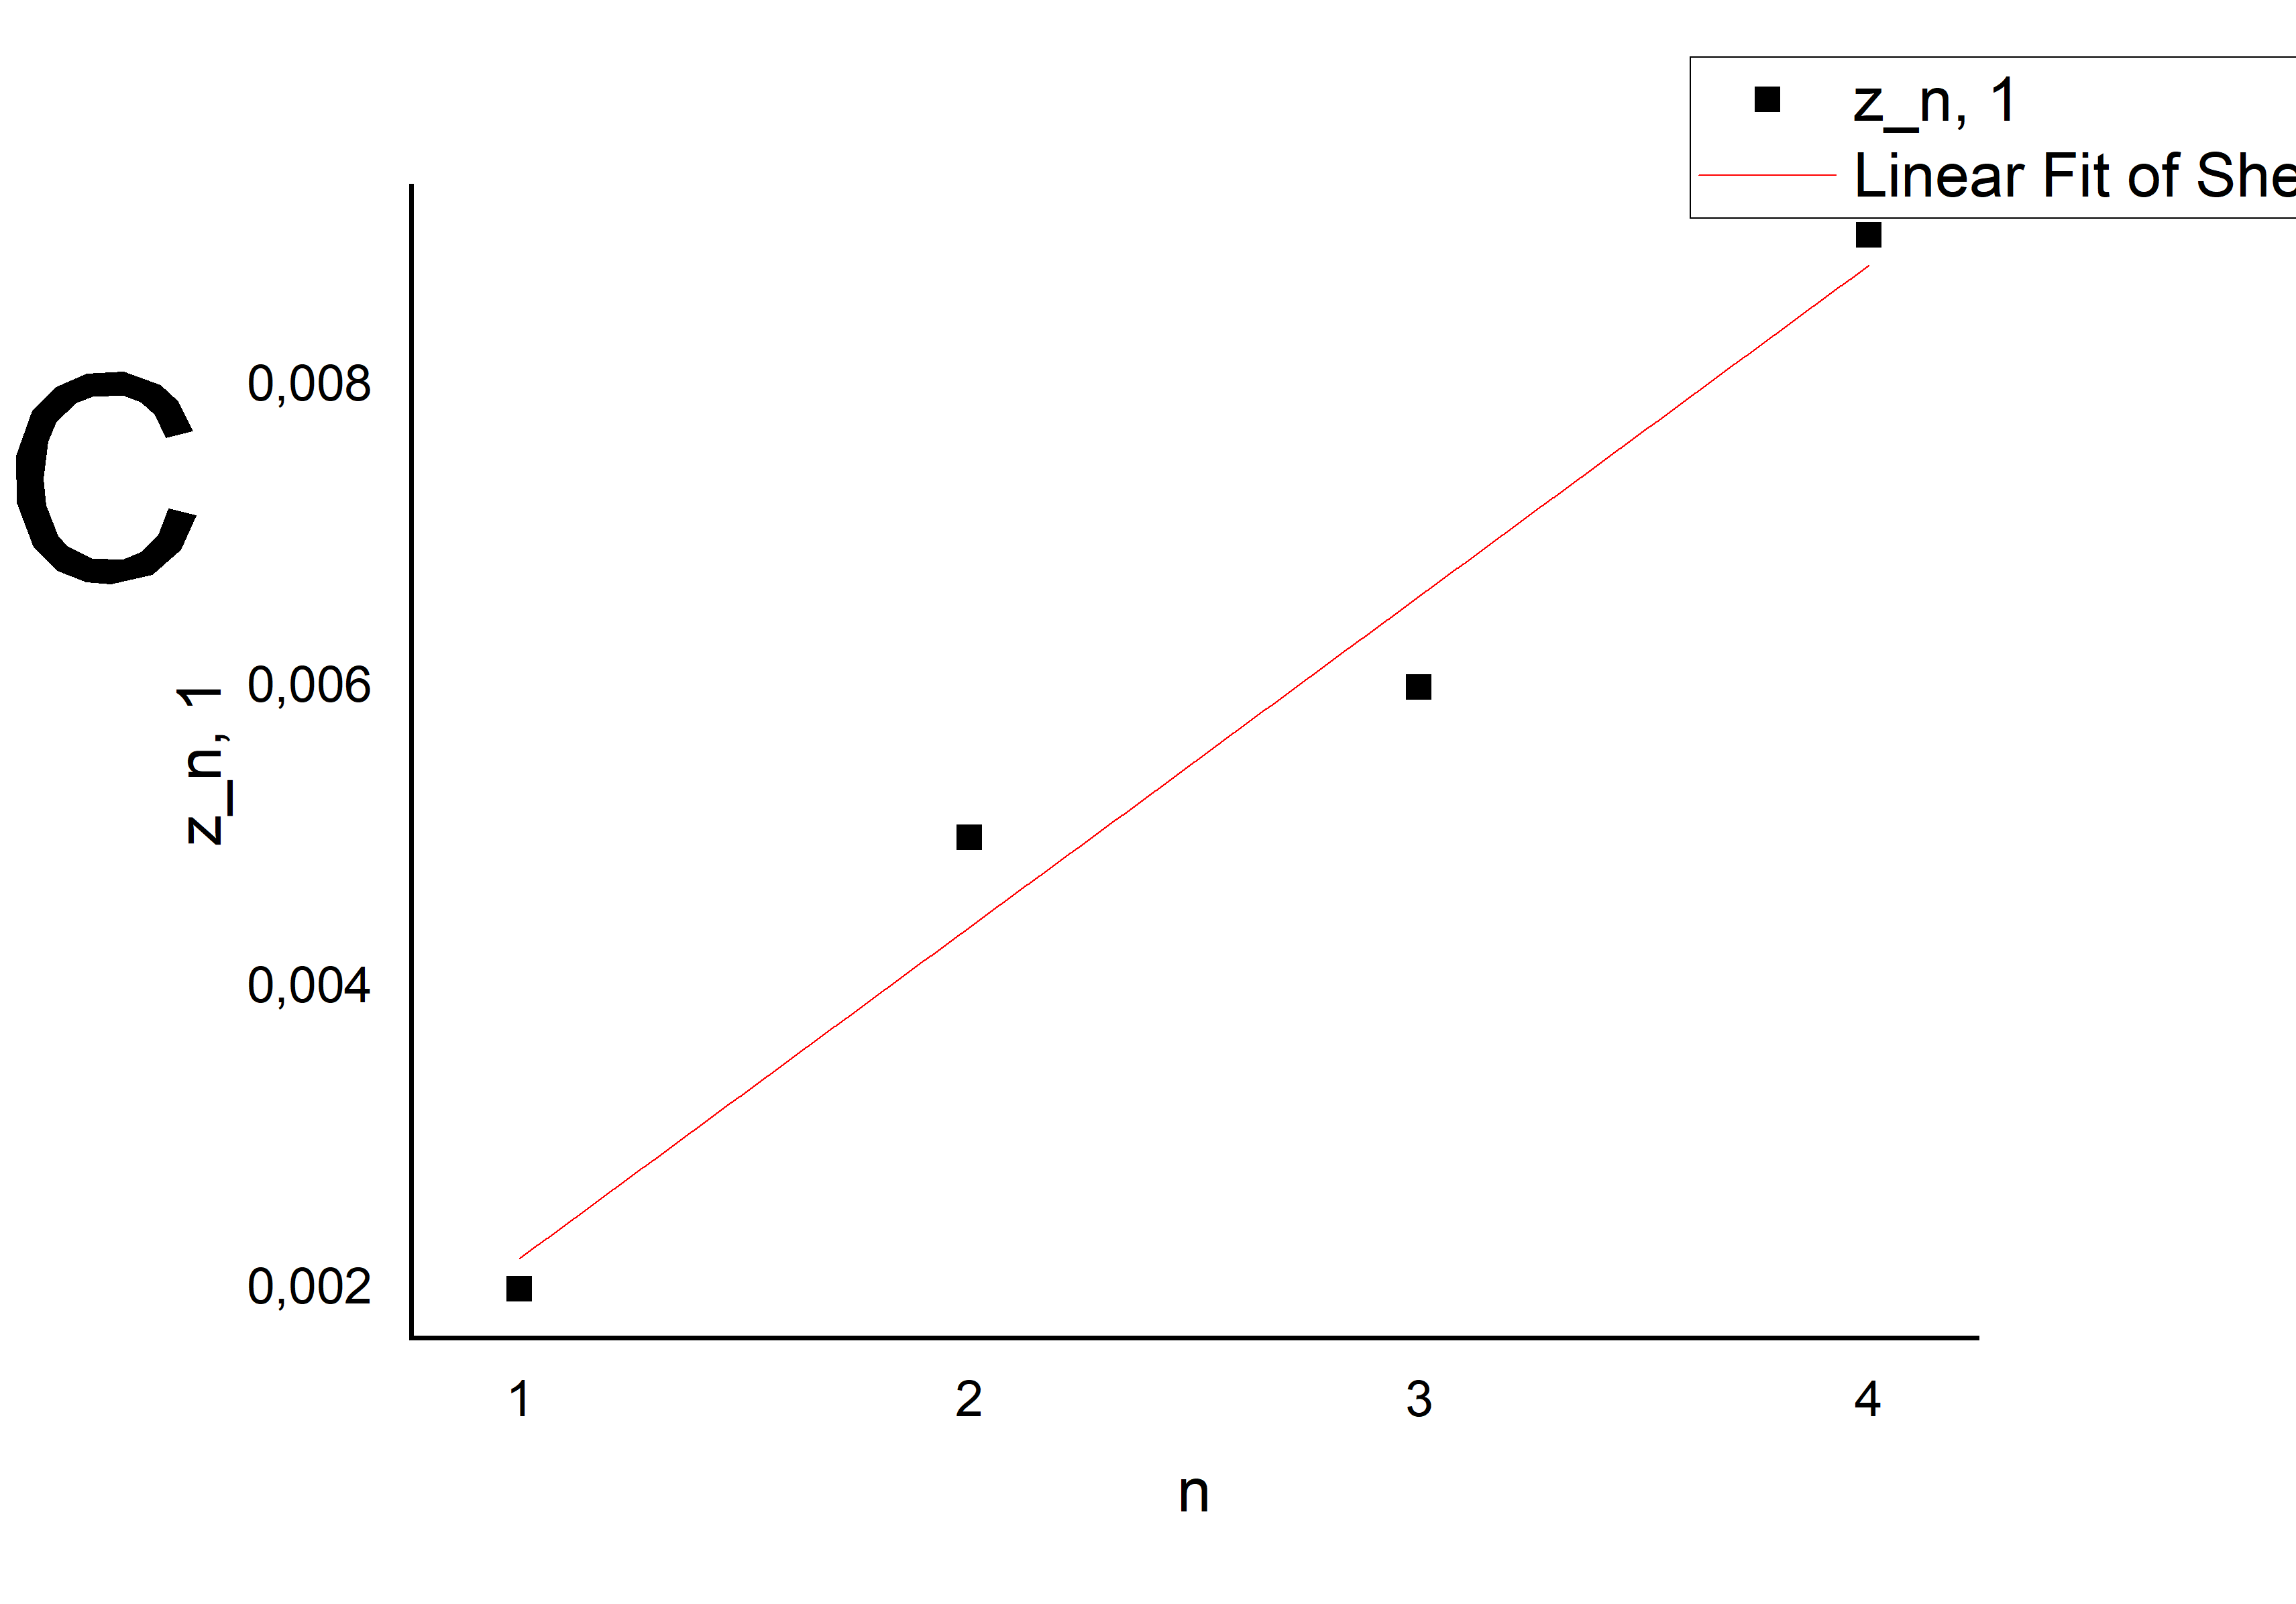
\includegraphics[scale=0.2]{1.png}\hfill
		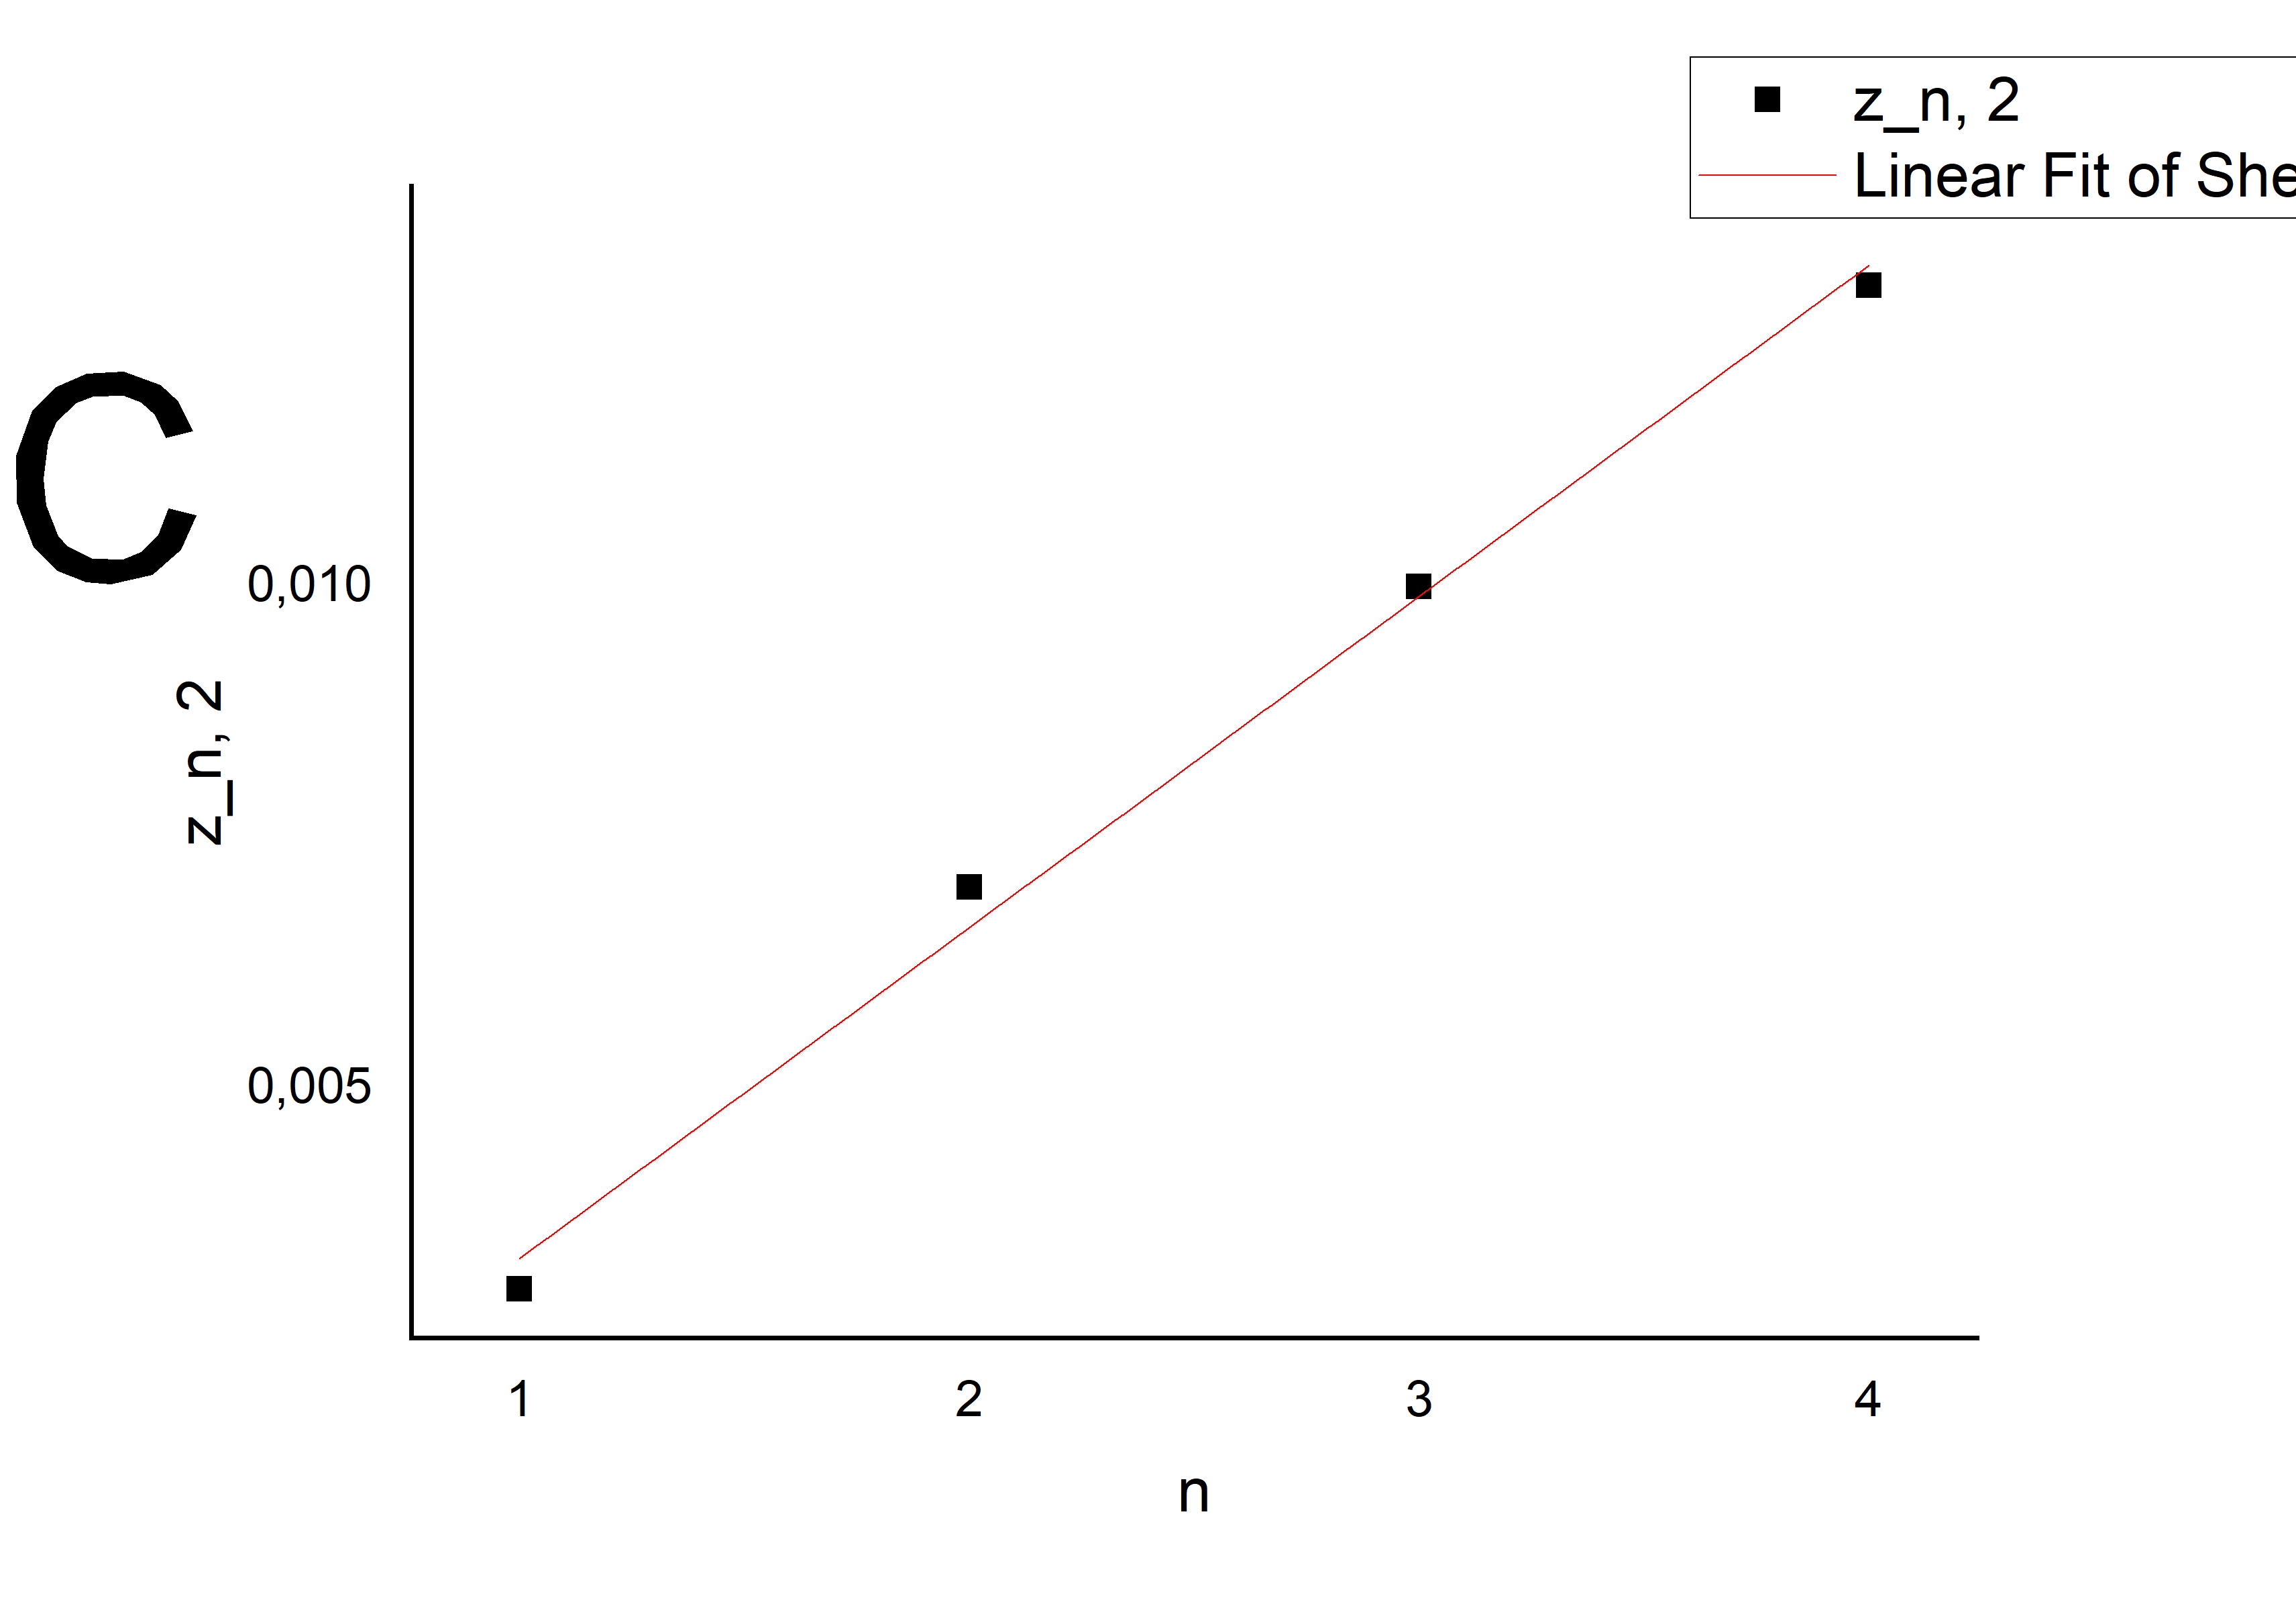
\includegraphics[scale=0.2]{2.png}\hfill
		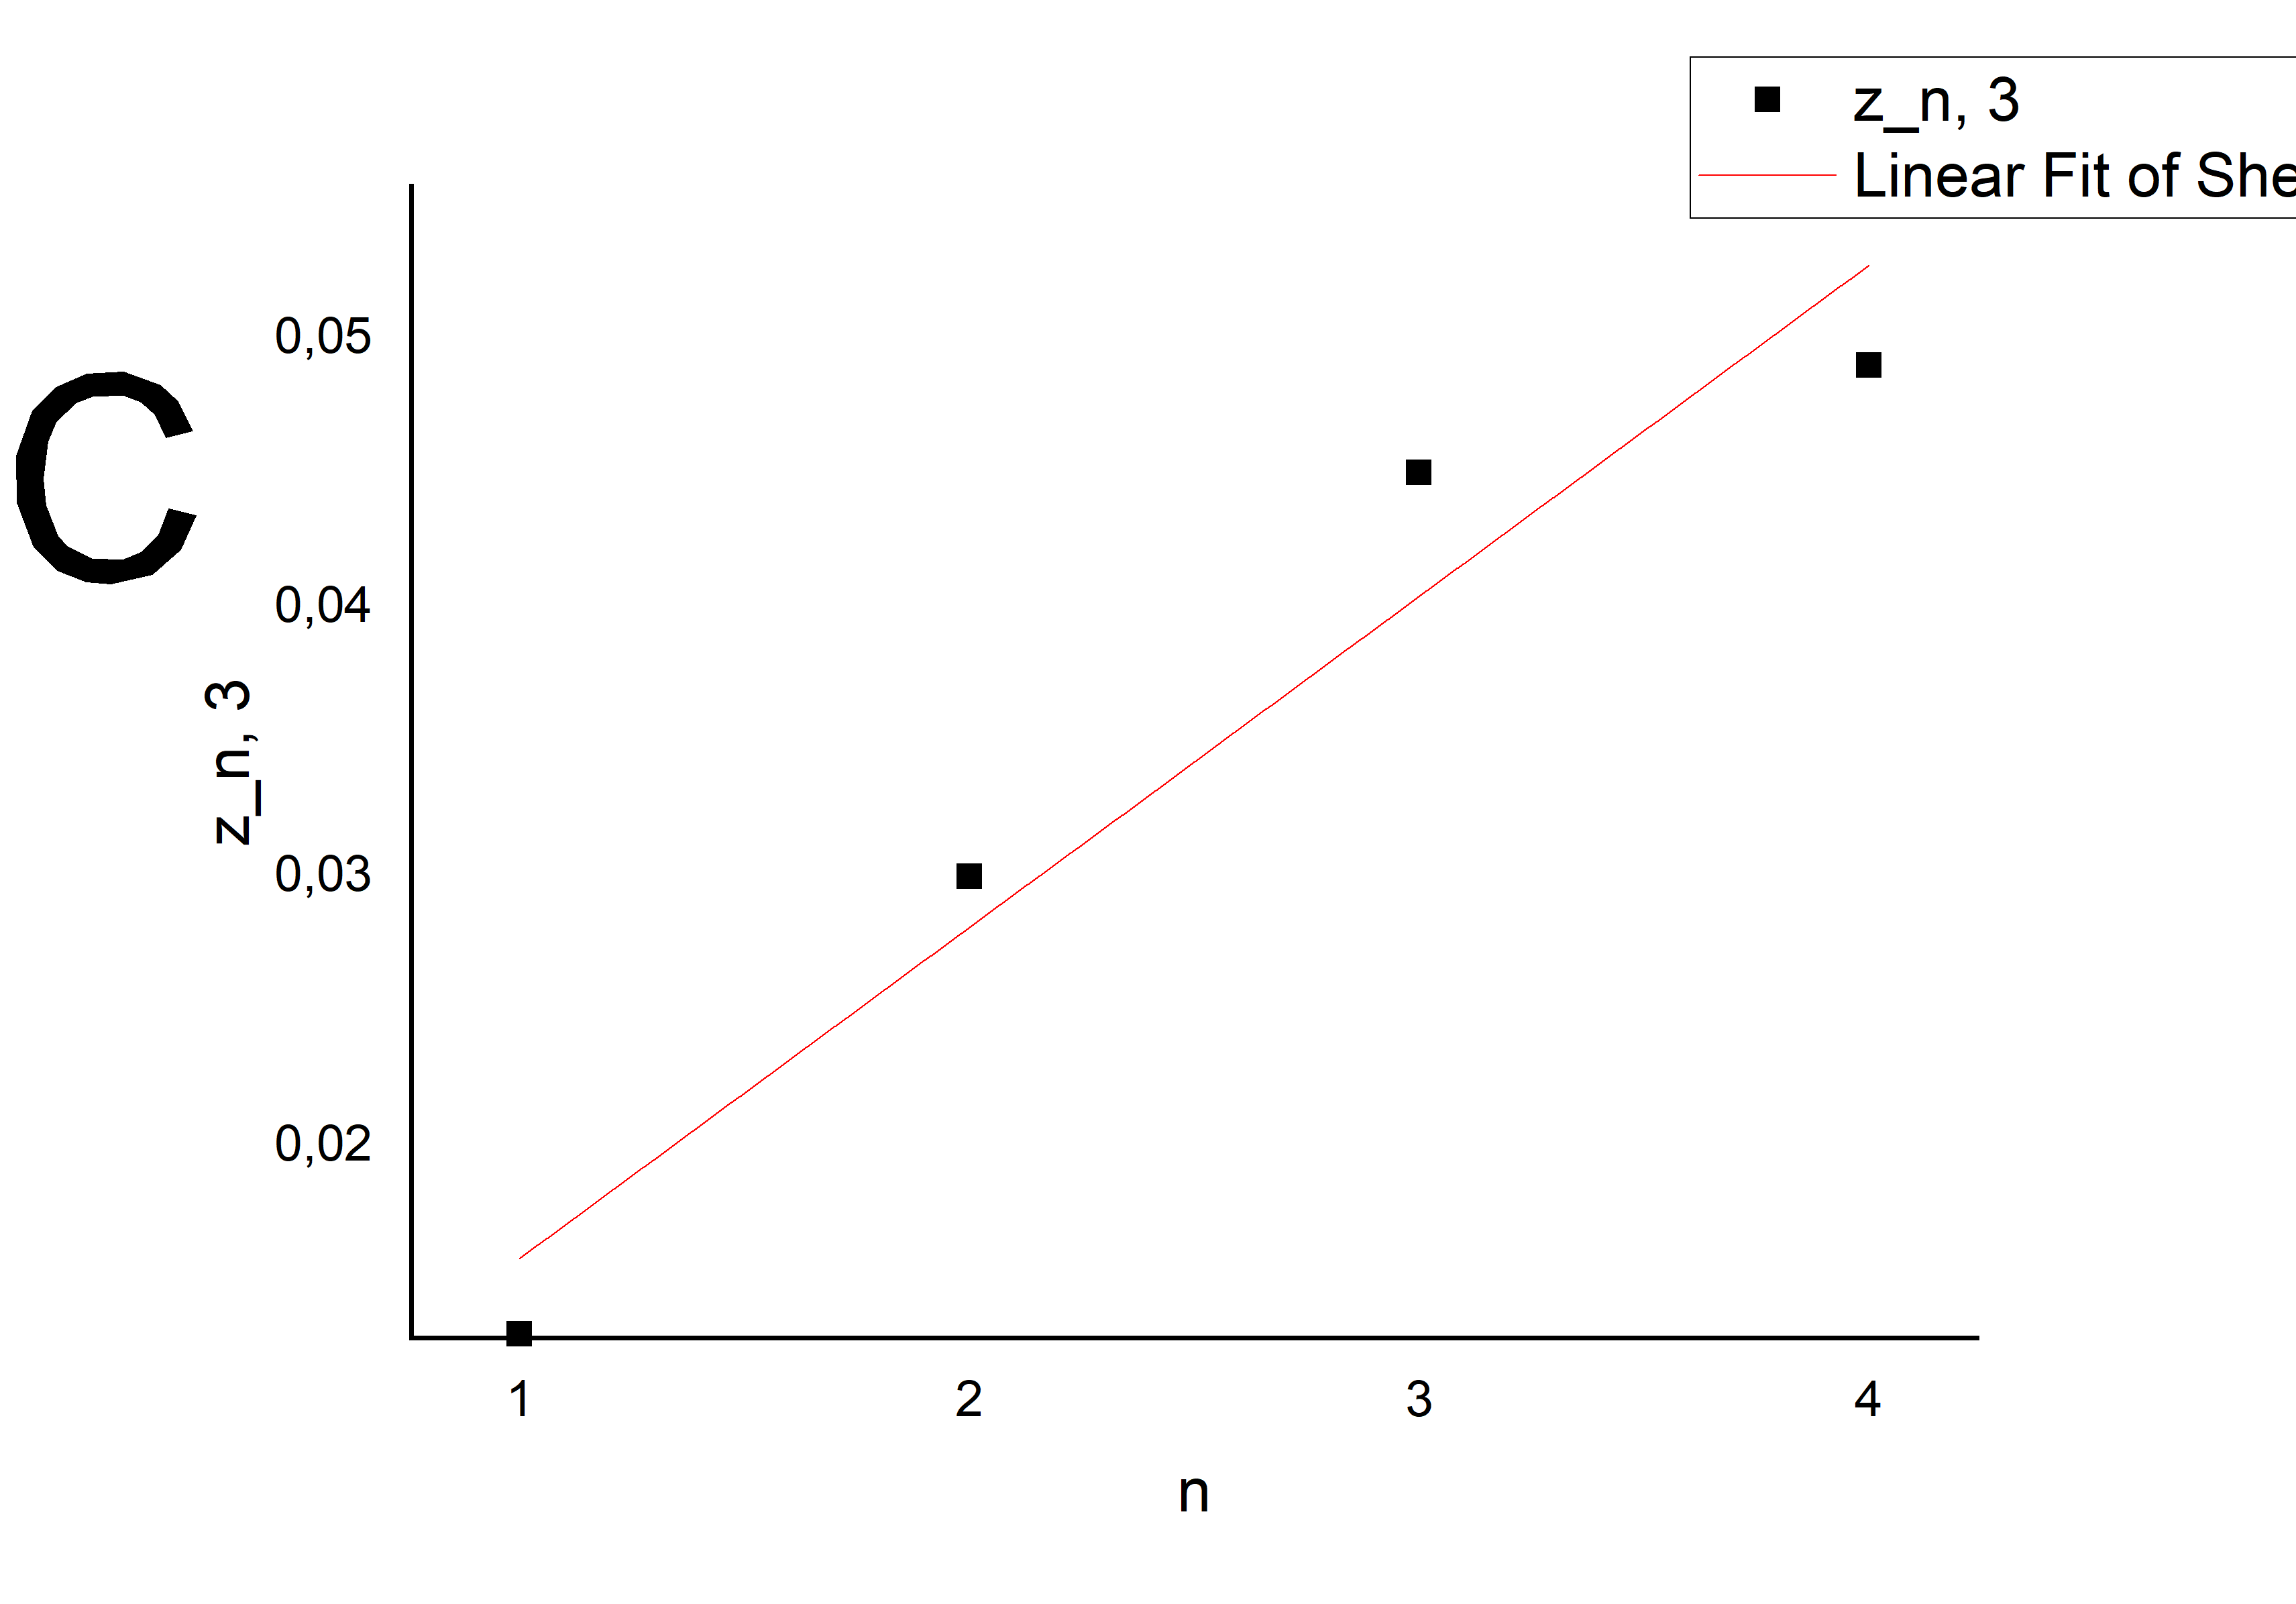
\includegraphics[scale=0.2]{3.png}\hfill
		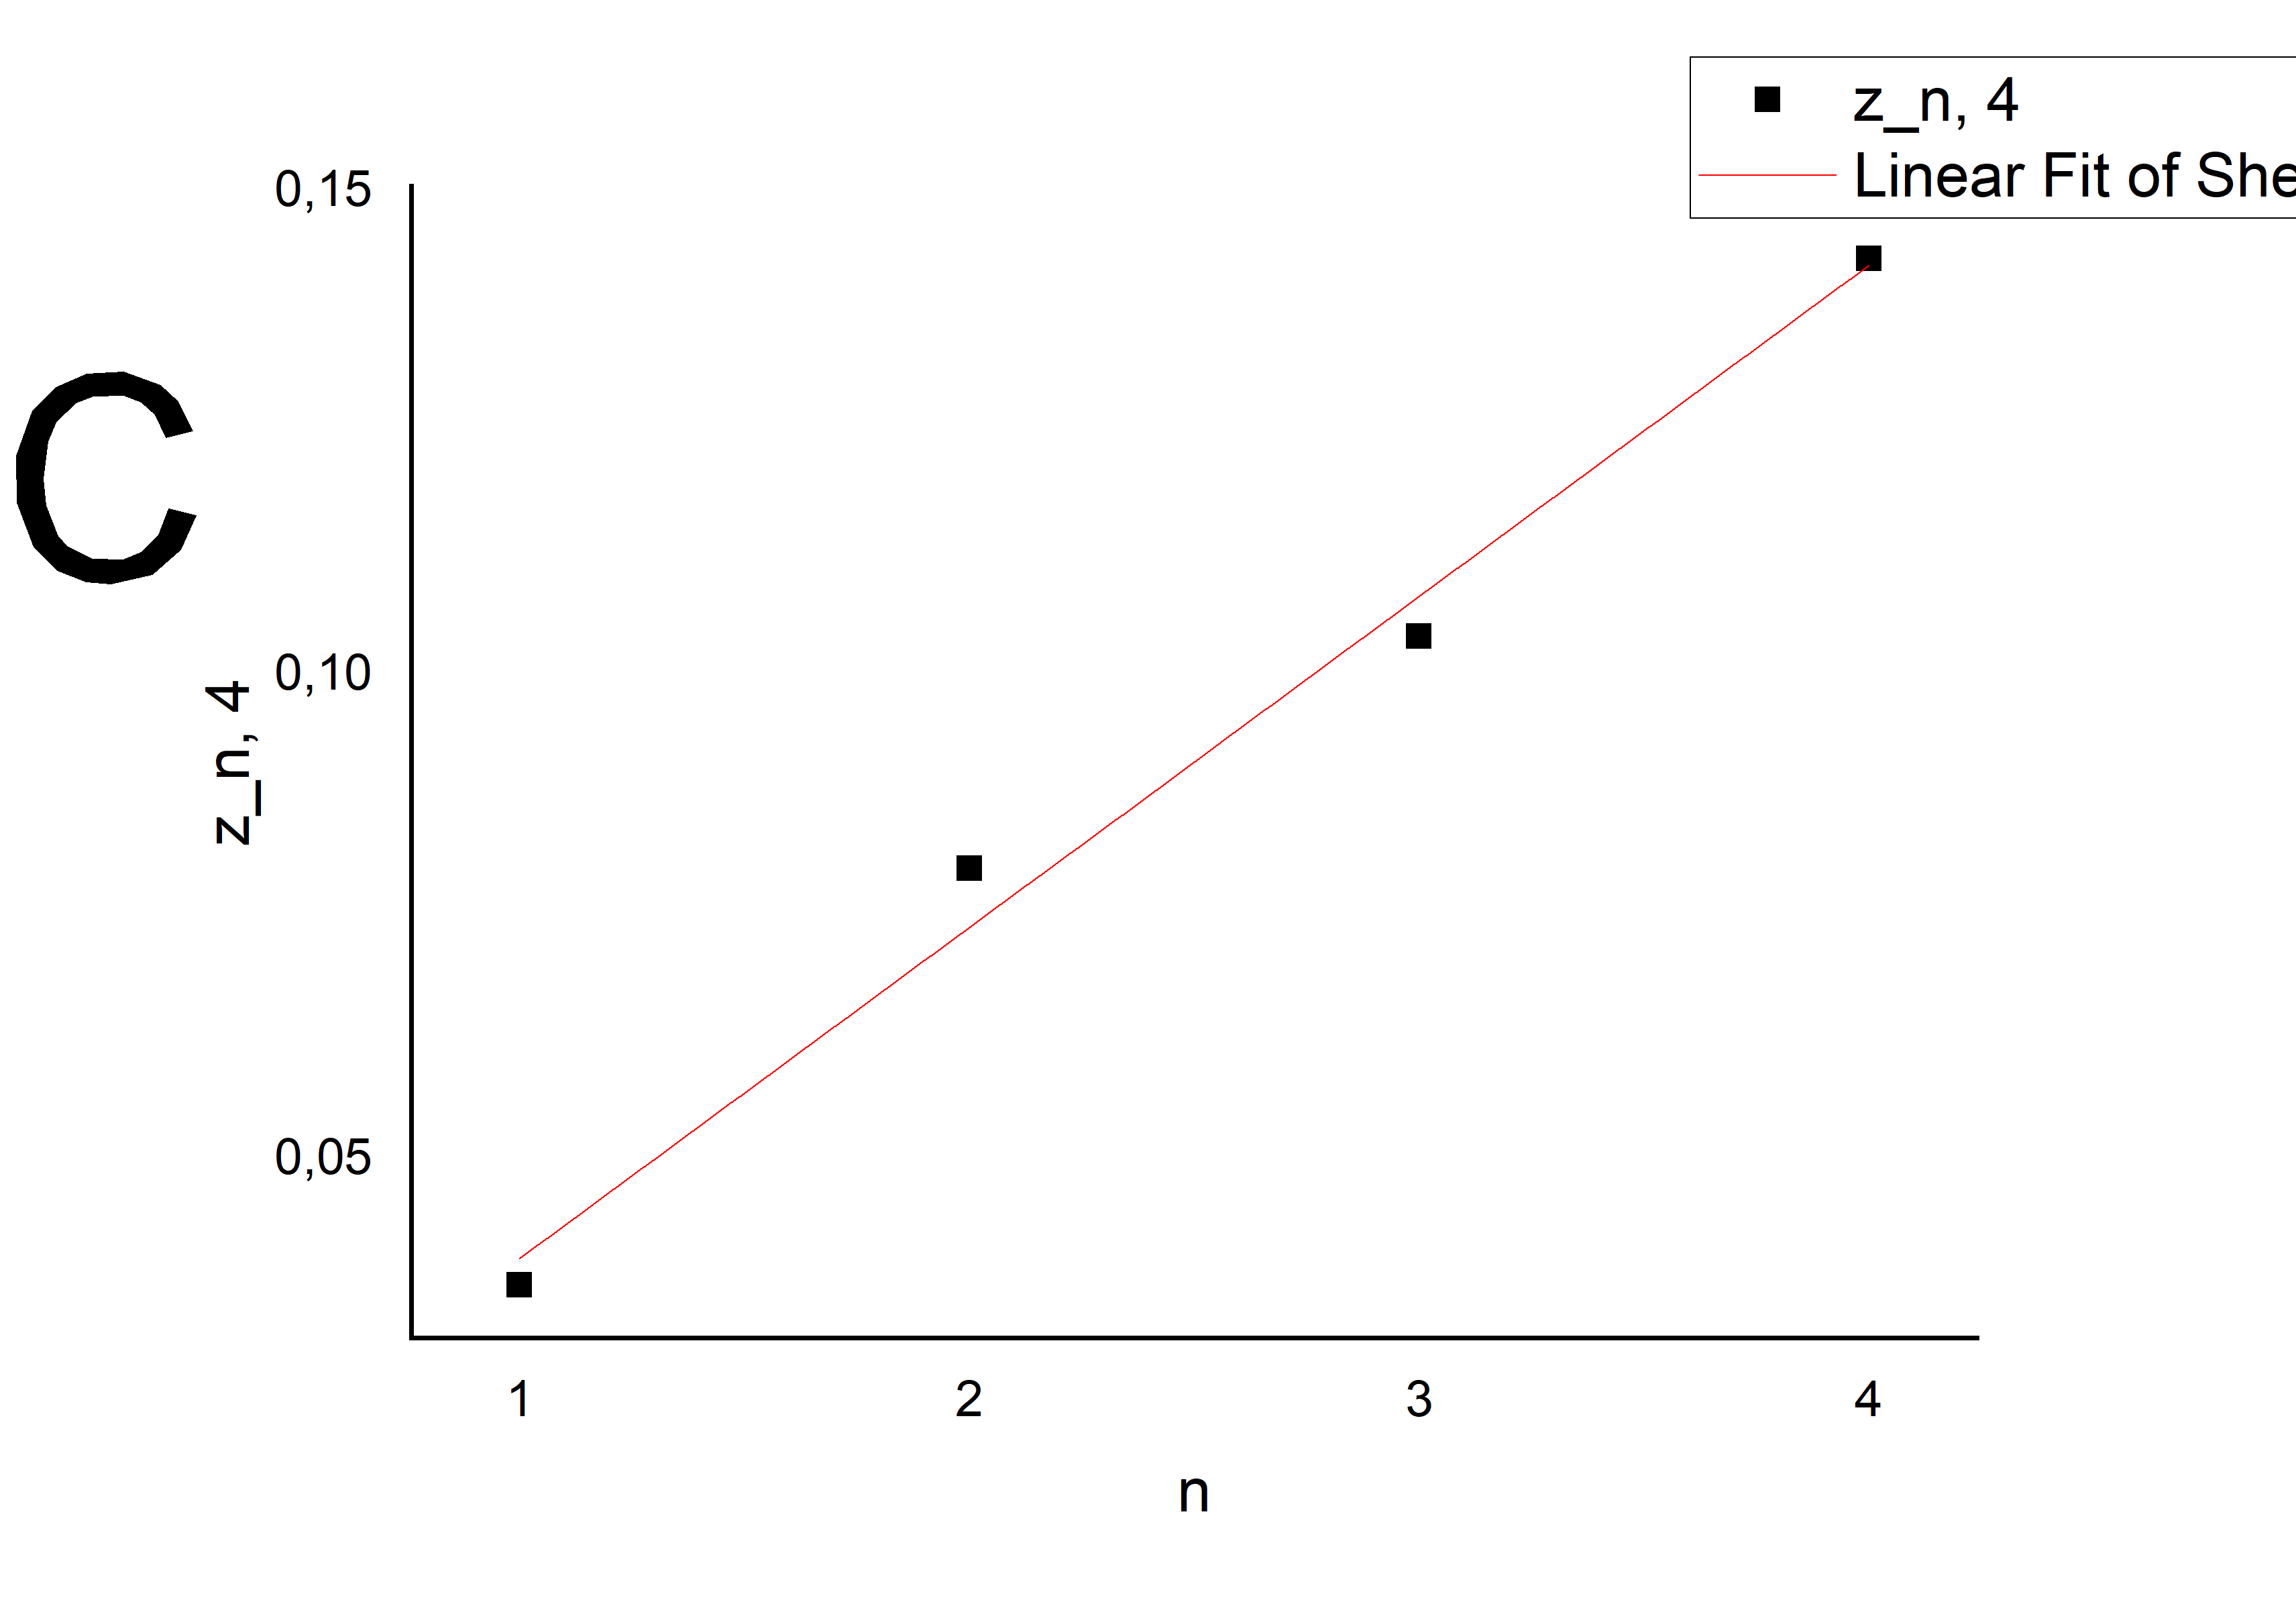
\includegraphics[scale=0.2]{4.png}\hfill
		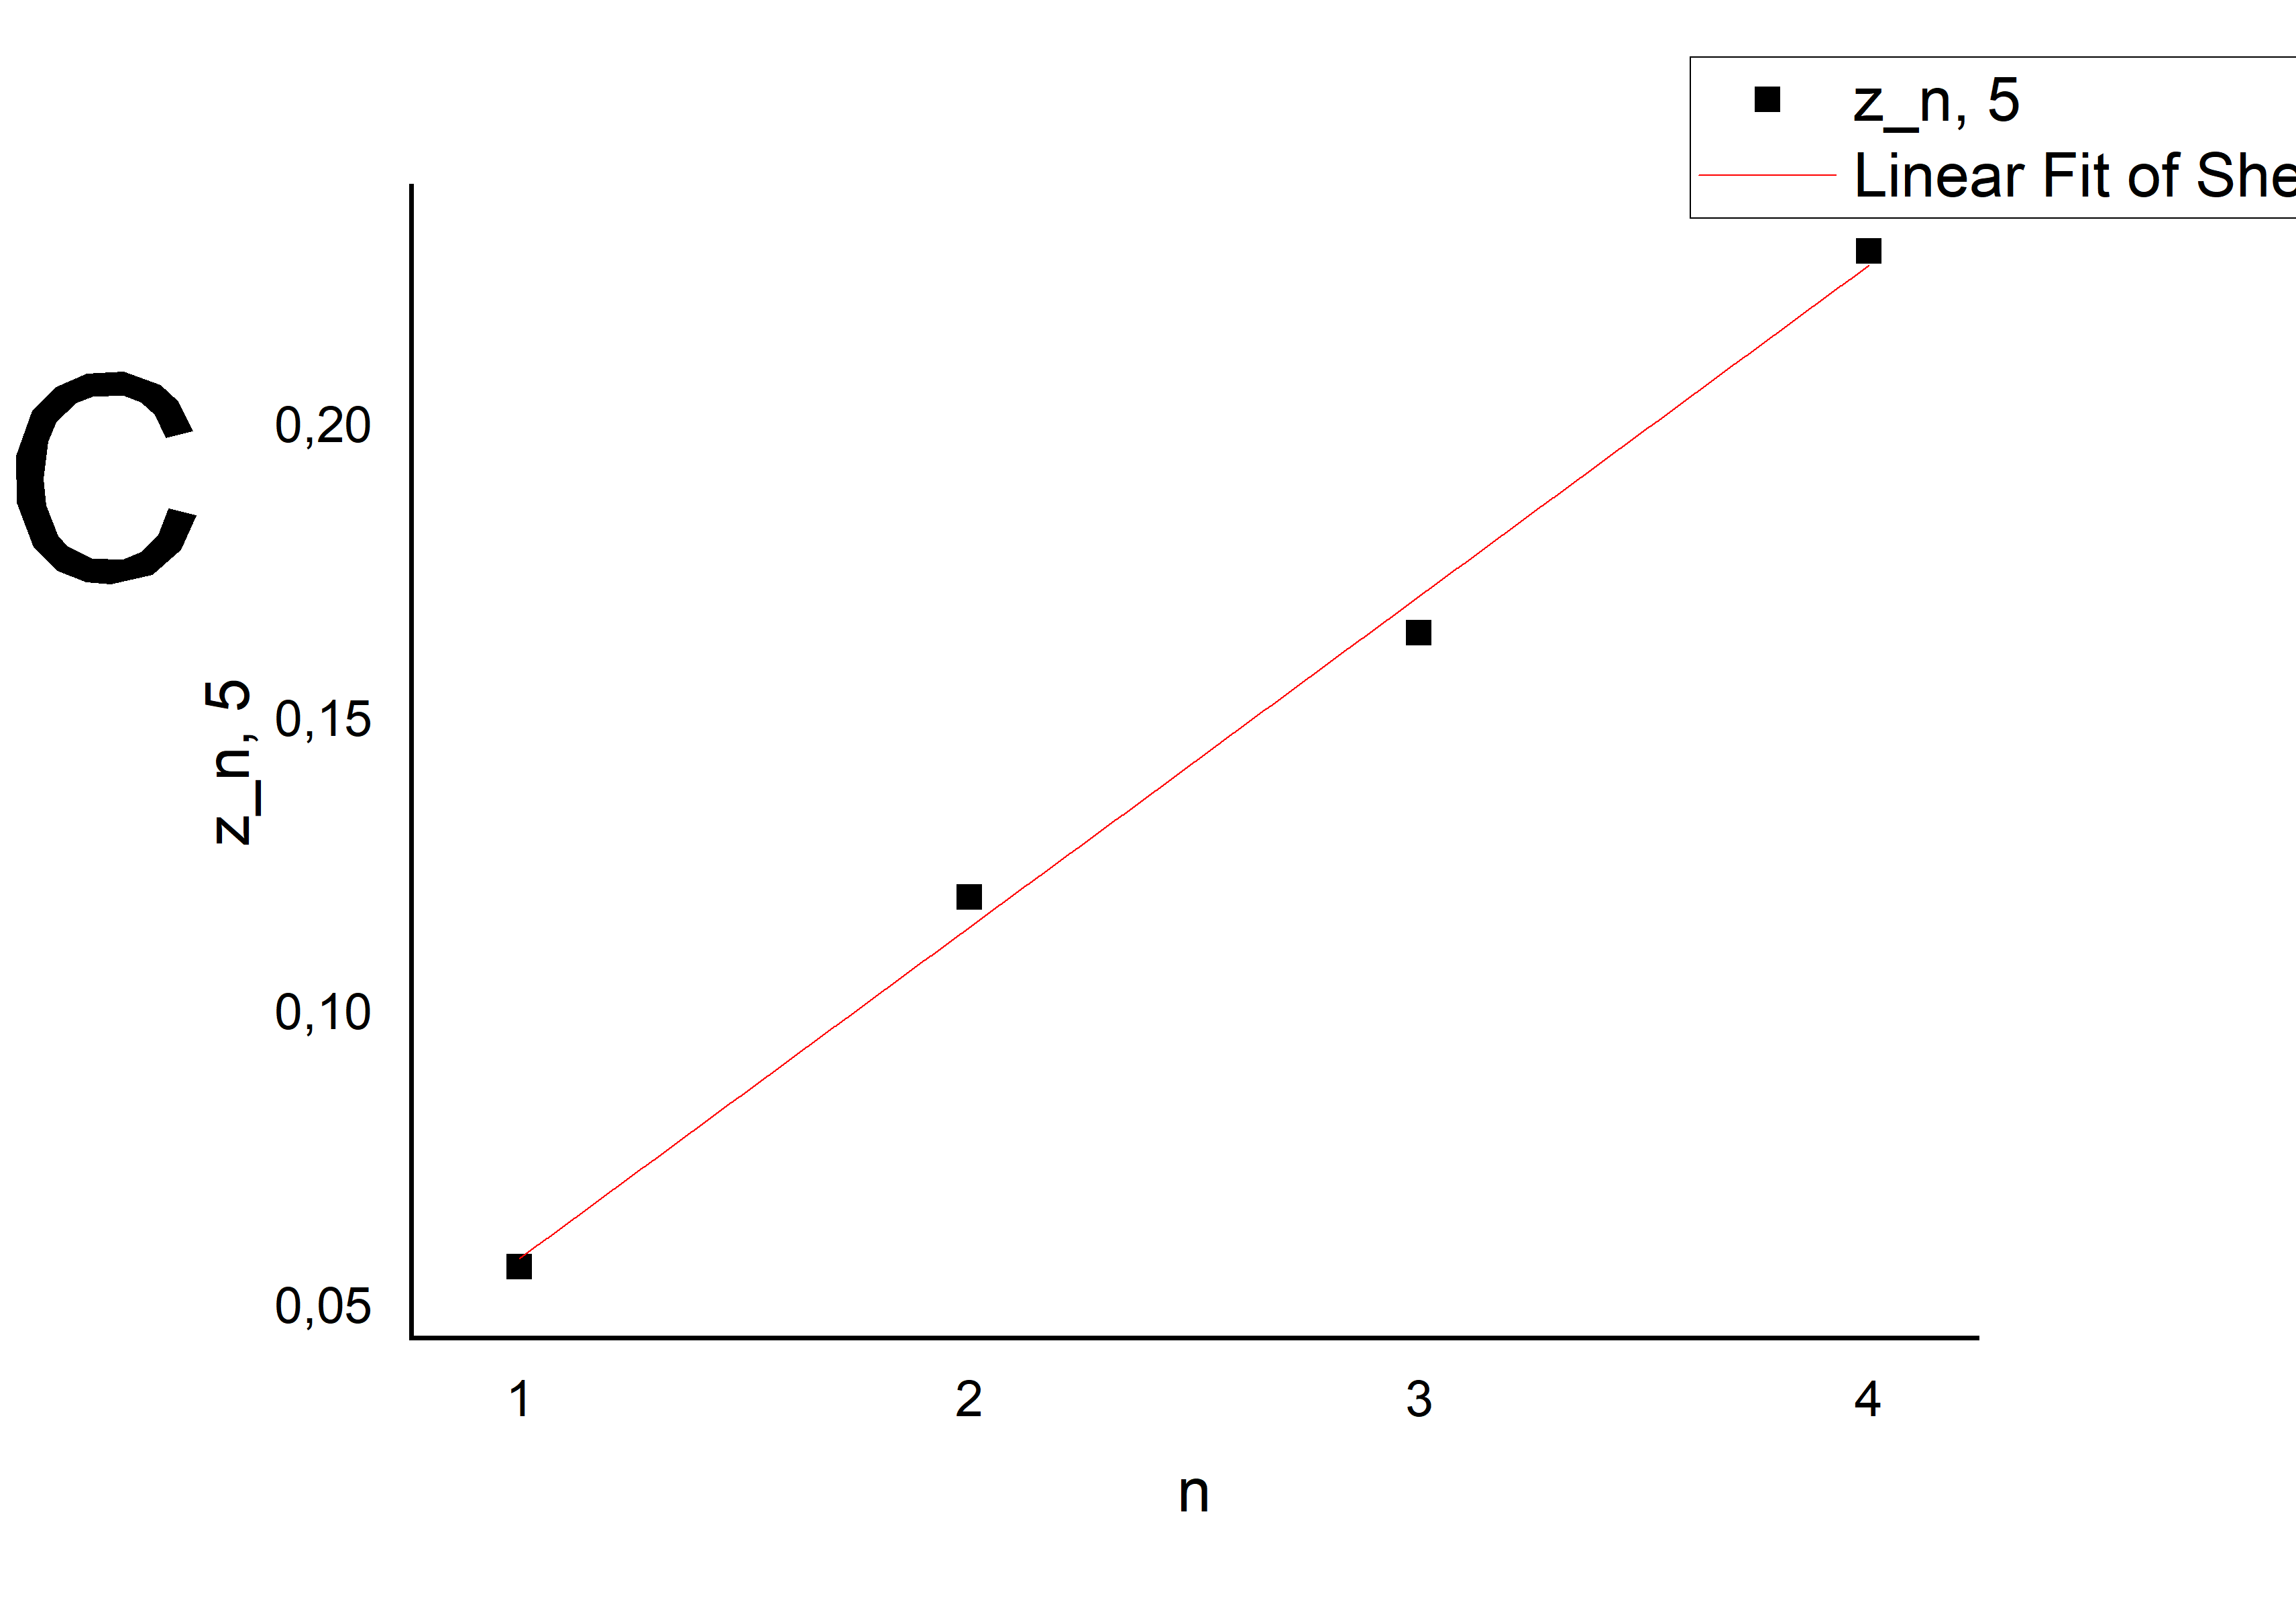
\includegraphics[scale=0.2]{5.png}
	\end{figure*}
\subsection{Мира}

Укажем таблицу с результатами измерений периода миры 25 с помощью линзы и изображения на экране:

\begin{table}[h!]
	\begin{tabular}{llll|l|lll}
		\hline
		\multicolumn{8}{|c|}{Измерение   периода миры 25 с помощью линзы и законов геометрической оптики}                                                                                                    \\ \hline
		\multicolumn{1}{|l|}{$a$, м}  & \multicolumn{1}{l|}{$b$, м} & \multicolumn{1}{l|}{$da$, м}  & $db$, м  & $L$, м   & \multicolumn{1}{l|}{$m$}  & \multicolumn{1}{l|}{$x$,м}      & \multicolumn{1}{l|}{$d$, м}        \\ \hline
		\multicolumn{1}{|l|}{0,054} & \multicolumn{1}{l|}{1,28} & \multicolumn{1}{l|}{0,0005} & 0,0005 & 0,018  & \multicolumn{1}{l|}{35} & \multicolumn{1}{l|}{0,000514} & \multicolumn{1}{l|}{2,16964E-05} \\ \hline
		&                           &                             &        & $dL$, м  &                         &                               &                                  \\ \cline{5-5}
		&                           &                             &        & 0,0005 &                         &                               &                                  \\ \cline{5-5}
	\end{tabular}
\end{table}
В этом случае получился период $d \approx 22$ микрона.
\newpage
Далее измеряем период с помощью саморепродукции. Получается таблица:
\begin{table}[h!]
	\begin{tabular}{|l|l|llllll}
		\hline
		\multicolumn{8}{|c|}{Измерение   периода миры 25 с помощью саморепродукции}                                                \\ \hline
		\multicolumn{5}{|c|}{$n$}                                                                                           &  &  &  \\ \cline{1-5}
		1         & 2           & \multicolumn{1}{l|}{3}      & \multicolumn{1}{l|}{4}      & \multicolumn{1}{l|}{5}      &  &  &  \\ \cline{1-5}
		\multicolumn{5}{|c|}{$z_n$}                                                                                        &  &  &  \\ \cline{1-5}
		0,0022    & 0,0051      & \multicolumn{1}{l|}{0,0079} & \multicolumn{1}{l|}{0,0112} & \multicolumn{1}{l|}{0,0142} &  &  &  \\ \cline{1-5}
		наклон, м & $d$, м        &                             &                             &                             &  &  &  \\ \cline{1-2}
		0,003     & 2,82489E-05 &                             &                             &                             &  &  &  \\ \cline{1-2}
	\end{tabular}
\end{table}
В этом случае получился период $d \approx 22$ микрона.
График саморепродукции, из которого был определен период $d$ по МНК: 
\begin{figure}[h!]
	\begin{center}
		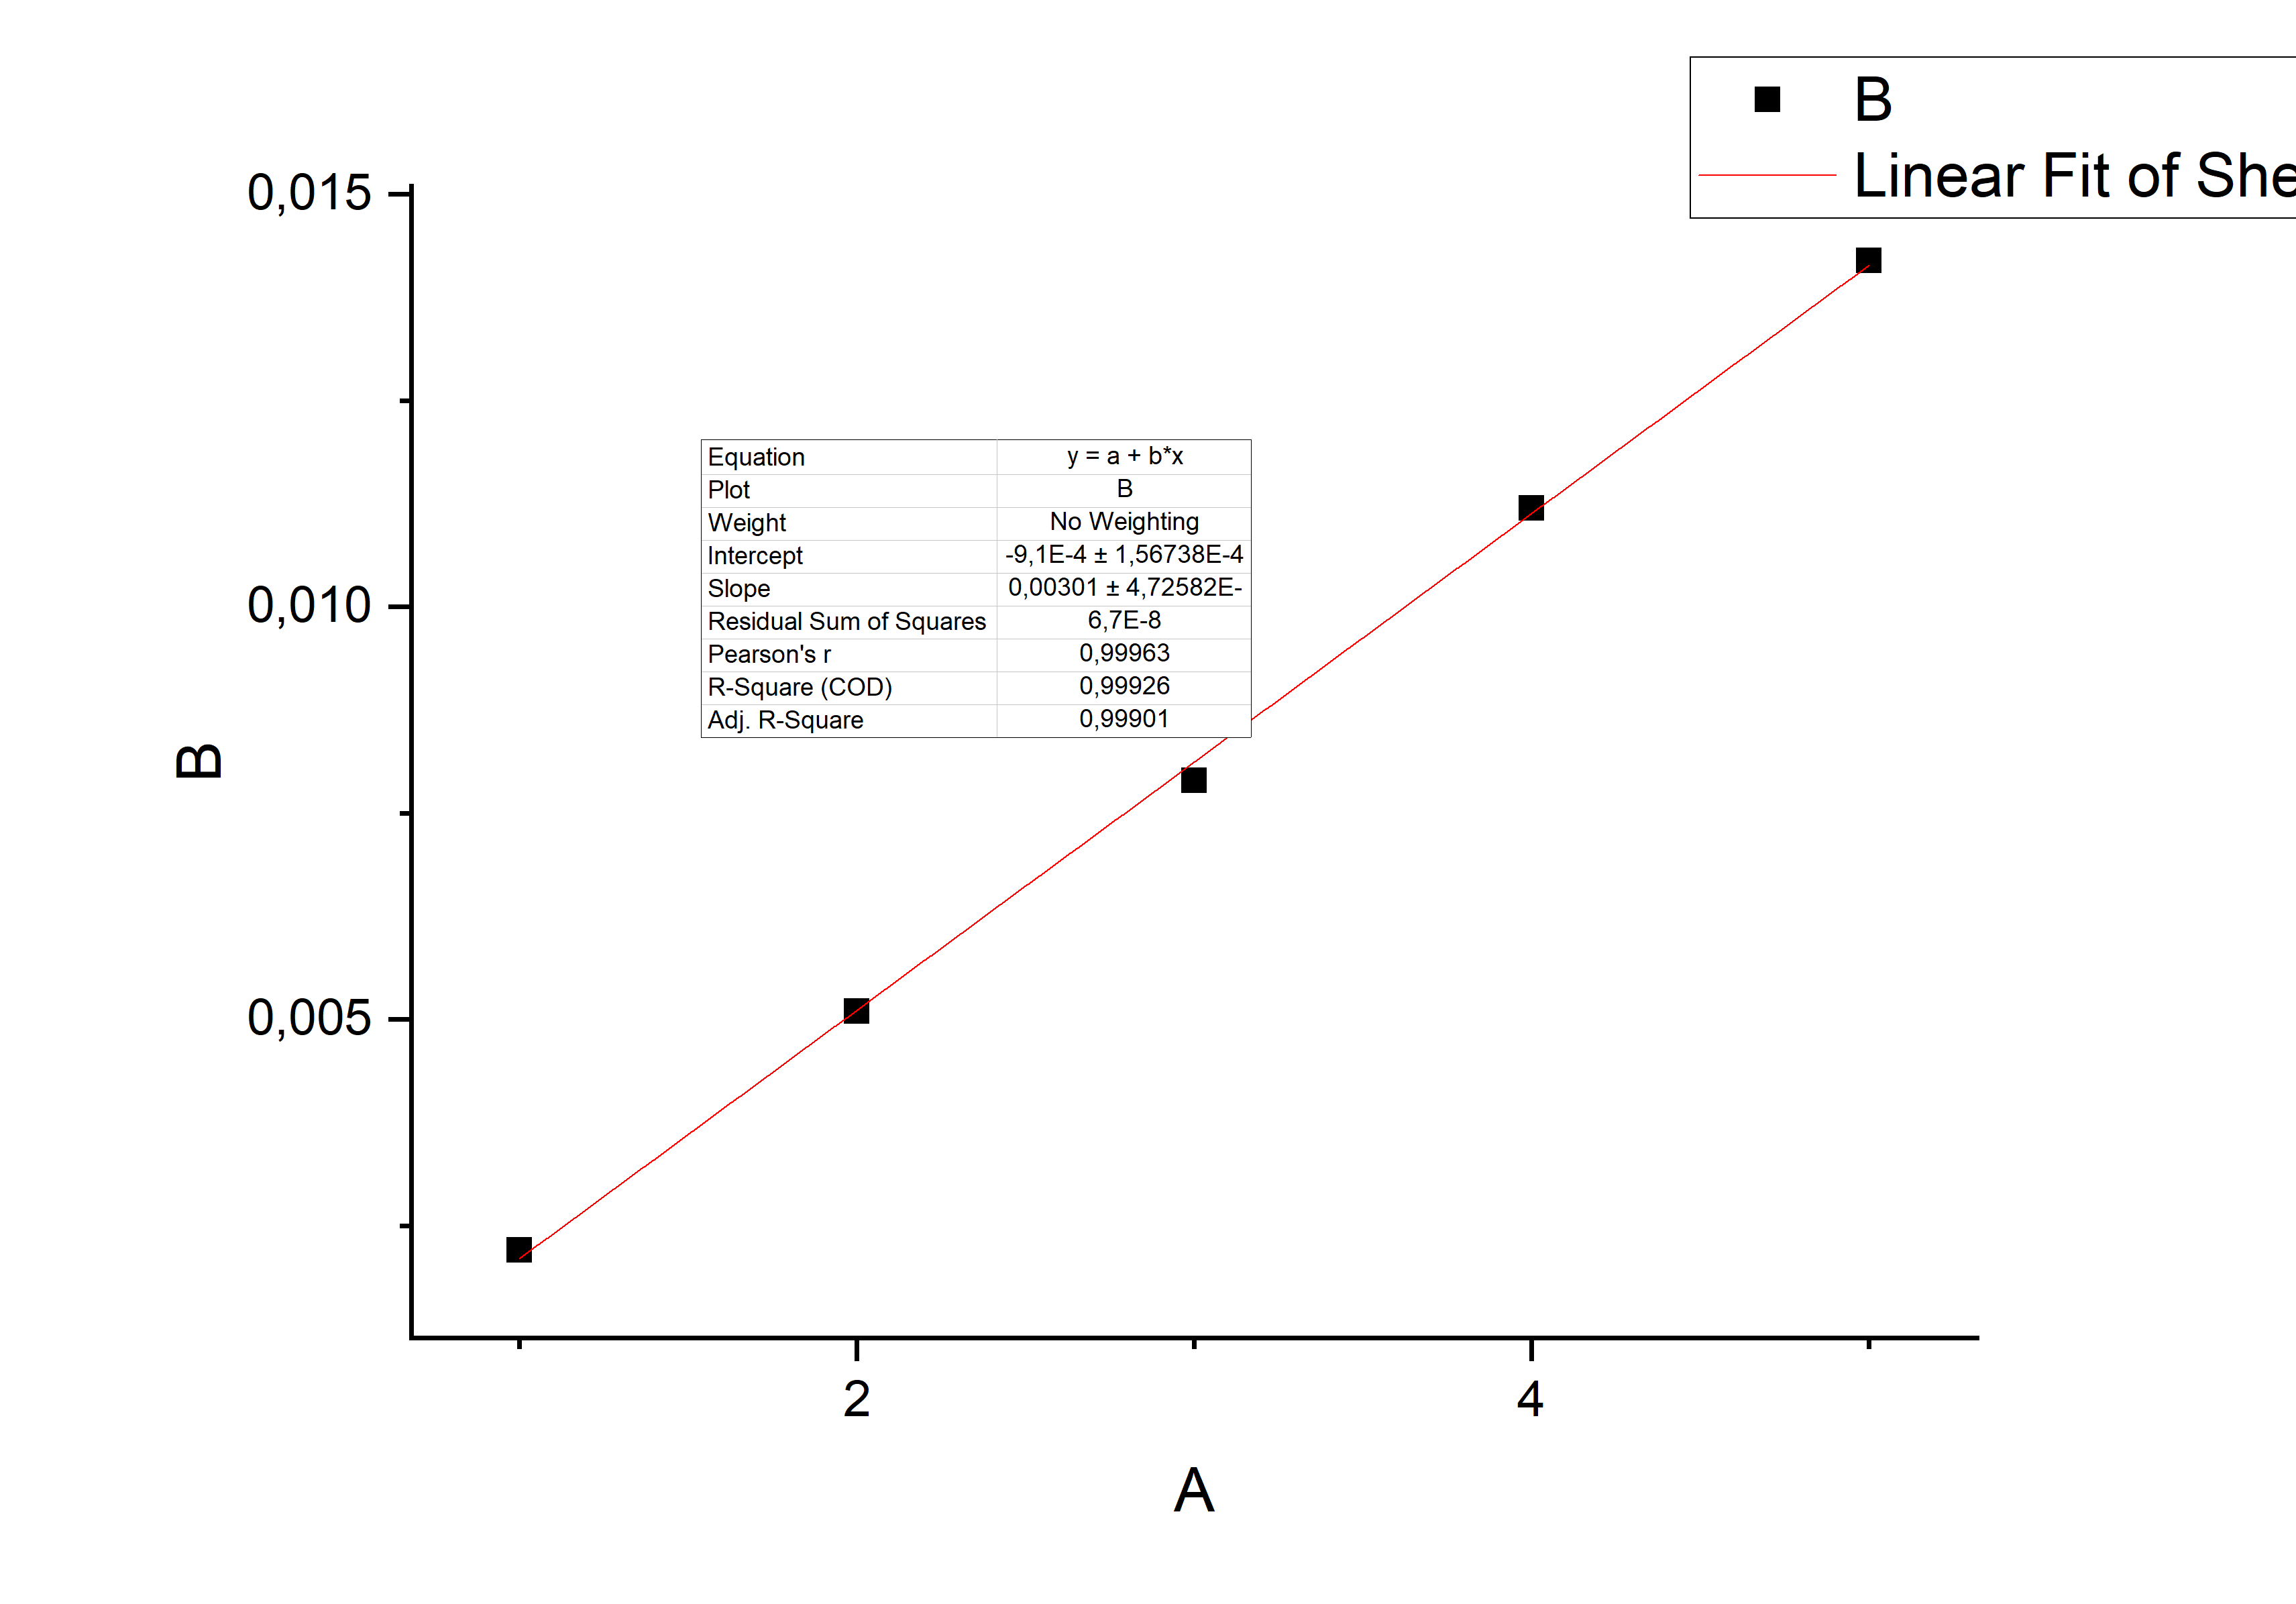
\includegraphics[scale = 0.4]{мира.png}
	\end{center}
\end{figure}

\section{Вывод}

В работе были измерены периоды решеток и миры тремя различными способами - везде были получены результаты, близкие друг к другу, что говорит об успешности проделанного эксперимента.
\end{document} % конец документа